% \documentclass[t]{beamer}
\documentclass{beamer}
\usepackage{minted}
\usepackage{tikz}
\usepackage{amsmath}
\usepackage{adjustbox}

\title{Synchronous single initiator spanning tree algorithm using flooding}
\author{Siddharth Bhat, Anurag Chaturvedi, Hitesh Kaushik}
\date{\today}

\begin{document}
\begin{frame}
\titlepage
\end{frame}

\begin{frame}
    % spanning tree computation: why is it hard in a distributed system
\end{frame}


% algorithm explanation
\begin{frame}
    \frametitle{Example}
    \begin{adjustbox}{min totalsize={.5\textwidth}{.5\textheight}}
    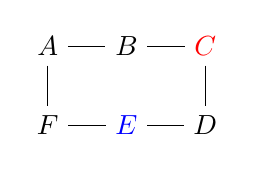
\begin{tikzpicture}
        \node (A) {$A$};
        \node (B) [right of = A] {$B$};
        \node (C) [right of = B, color=red] {$C$};
        \node (D) [below of = C] {$D$};
        \node (E) [below of = B, color=blue] {$E$};
        \node (F) [below of = A] {$F$};

        \path (A) edge (B); 
        \path (A) edge (F);
        % 
        \path (B) edge (C);
        %
        \path (C) edge (D);
        % \path[thick] (C) edge (E);
        %\path [->, bend left] (C) to node{bar} (E);
        % 
        \path (D) edge (E);
        %
        \path (E) edge (F);
    \end{tikzpicture}
    \end{adjustbox}
\end{frame}

\begin{frame}
    \frametitle{Example}
    \begin{adjustbox}{min totalsize={.5\textwidth}{.5\textheight}}
    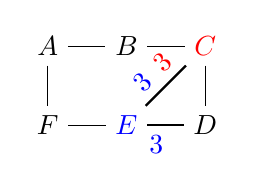
\begin{tikzpicture}
        \node (A) {$A$};
        \node (B) [right of = A] {$B$};
        \node (C) [right of = B, color=red] {$C$};
        \node (D) [below of = C] {$D$};
        \node (E) [below of = B, color=blue] {$E$};
        \node (F) [below of = A] {$F$};

        \path (A) edge (B); 
        \path (A) edge (F);
        % 
        \path (B) edge (C);
        %
        \path (C) edge (D);
        % \path[thick] (C) edge (E);
        %\path [->, bend left] (C) to node{bar} (E);
        % 
        \path (D) edge (E);
        %
        \path (E) edge (F);
        \draw[thick] (E) -- (C) 
            node [near start, style={sloped}, anchor=south, color=blue]{3}
            node [near end, style={sloped}, anchor=south, color=red]{3};

        \draw[thick] (E) -- (D) 
            node [near start, anchor=north, color=blue]{3};
    \end{tikzpicture}
    \end{adjustbox}
\end{frame}

\begin{frame}[fragile]
    \frametitle{Synchronous BFS (Pseudocode)}
    \begin{itemize}
        \item Assume root begins computation.
        \item Algorithm is synchronous.
    \end{itemize}
    \pause

    \begin{minted}{python}
    def bfs_spanning_tree(self):
    \end{minted}
    \pause
    \begin{minted}{python}
      if self.id == ROOT_ID:
        self.visited = True; self.depth = 0;
        for n in self.neighbours: n.send(self.id)
    \end{minted}
    \pause
    \begin{minted}{python}
      for round in range(1, DIAMETER+1):
        if self.visited: # if visited, skip
    \end{minted}
    \pause
    \begin{minted}{python}
          if self.queries: # if we have a query
            # randomly choose from queries
            parent = random.choice(self.query)
            self.visited = True
            self.depth = round
    \end{minted}
    \pause
    \begin{minted}{python}
            # synchronous
            for n in self.neighbours: n.send(self.id)
        self.queries = [];
    \end{minted}
\end{frame}

\begin{frame}
    % Thank you (backup slides after this)
\end{frame}

\begin{frame}
    % Minimum weight spanning tree: synchronous (5.5.11, Kshemkalyani)
\end{frame}

\begin{frame}
    % Spanning tree computation: async version
\end{frame}


\begin{frame}
    % Converting bounded delay to synchronous (Gerard Tel, Chapter 12)
\end{frame}

\end{document}
